\RequirePackage[orthodox]{nag}
\documentclass[11pt]{article}

%% Define the include path
\makeatletter
\providecommand*{\input@path}{}
\g@addto@macro\input@path{{include/}{../include/}}
\makeatother

\usepackage{../../include/akazachk}


\title{ECH4905 ChemE Optimization HW 6}
\author{Andres Espinosa}

\begin{document}
\maketitle

\section{Problem 1}
Consider the following problem:

\[
\text{minimize } 
\begin{aligned}
    Z_1(\mathbf{x}) &= x_1^2 + x_2^2 + x_3^2 + x_4^2 + x_5^2, \\
    Z_2(\mathbf{x}) &= 3x_1 + 2x_2 - x_3^3 + 0.01(x_4 - x_5)^3,
\end{aligned}
\]

\[
\text{subject to:}
\]
\[
\begin{aligned}
    x_1 + 2x_2 - x_3 - 0.5x_4 + x_5 &= 2, \\
    4x_1 - 2x_2 + 0.8x_3 + 0.6x_4 + 0.5x_5^2 &= 0, \\
    x_1^2 + x_2^2 + x_3^2 + x_4^2 + x_5^2 &\leq 10.
\end{aligned}
\]

\subsection{Part A}
Use the epsilon-constraint method to solve the above nonlinear programming (NLP) problem in GAMS. Upload your code.

\textbf{Solution:}
To solve this with the epsilon-constraint method, we can take the first objective $Z_1$ and set that as our primary objective, while we take the second objective $Z_2$ and turn that into a constraint.
The optimization problem now looks like this:

\begin{align*}
  \text{minimize} & \quad Z_1(\textbf{x}) = x_1^2 + x_2^2 + x_3^2 + x_4^2 + x_5^2 \\
  \text{subject to} & \quad x_1 + 2x_2 - x_3 - 0.5x_4 + x_5 = 2, \\
  & \quad 4x_1 - 2x_2 + 0.8x_3 + 0.6x_4 + 0.5x_5^2 = 0, \\
  & \quad x_1^2 + x_2^2 + x_3^2 + x_4^2 + x_5^2 \leq 10 \\
  & \quad 3x_1 + 2x_2 - x_3^3 + 0.01(x_4 - x_5)^3 \leq \varepsilon
\end{align*}
Below is the GAMS code that was used for this problem.
\begin{verbatim}
Sets
n / 1*30 /;

Parameters
epsilon_n(n)
pareto_z1(n)
pareto_z2(n);

Scalars
    z2_min
    z2_max
    epsilon /1/;


Variables
x_1
x_2
x_3
x_4
x_5
z_1
z_2;

x_1.lo = -4;   x_1.up = 4;
x_2.lo = -4;   x_2.up = 4;
x_3.lo = 0;   x_3.up = 4;
x_4.lo = -4;   x_4.up = 4;
x_5.lo = -4;   x_5.up = 4;

z_1.lo = -1000; z_1.up = 1000;
z_2.lo = -1000; z_2.up = 1000;


Equations
z_1_eq
z_2_eq
constraint_1
constraint_2
constraint_3
non_neg_power_constraint
epsilon_constraint
;
z_1_eq.. z_1 =e= x_1**2 + x_2**2 + x_3**3 + x_4**2 + x_5**2;
z_2_eq.. z_2 =e= 3*x_1 + 2*x_2 - x_3**3 + 0.01*(x_4 - x_5)**3;
constraint_1.. x_1 + 2*x_2 - x_3 - 0.5*x_4 + x_5 =e= 2;
constraint_2.. 4*x_1 - 2*x_2 + 0.8*x_3 + 0.6*x_4 + 0.5*x_2**2 =e= 0;
constraint_3.. z_1 =l= 10;
non_neg_power_constraint.. x_4 =g= x_5;
epsilon_constraint.. z_2 =l= epsilon;

Model FullModel / all / ;
model BoundedModel / all - epsilon_constraint / ;

option NLP=baron;
option optcr = 0.00001;
option limrow = 4000;

* First, solve BoundedModel to get min and max z_2
solve BoundedModel using MINLP minimizing z_1;
z2_min = z_2.l;

solve BoundedModel using MINLP minimizing z_2;
z2_max = z_2.l;

* Now loop to build Pareto front
loop(n,
    epsilon_n(n) = z2_min + (z2_max - z2_min)*(ord(n)-1)/(card(n)-1);
    epsilon = epsilon_n(n);
    solve FullModel using MINLP minimizing z_1;
    pareto_z1(n) = z_1.l;
    pareto_z2(n) = z_2.l;
);

* Save results
execute_unload 'pareto_front.gdx', pareto_z1, pareto_z2, epsilon_n;
\end{verbatim}
\subsection{Part B}
Create a plot with the Pareto front.

\textbf{Solution:} 
The plot is available in Figure~\ref{fig:prob1_pareto}

\begin{figure}[htbp]
  \centerline{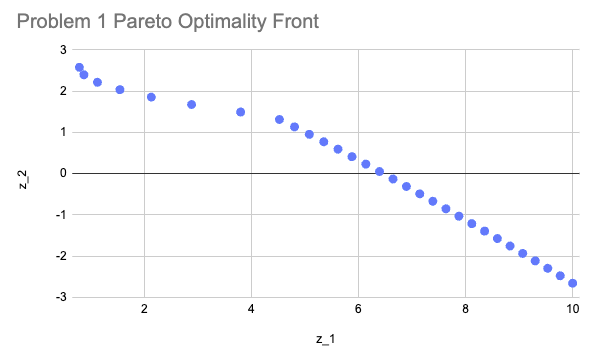
\includegraphics[width=0.75\textwidth]{images/prob1_pareto.png}}
  \caption{Problem 1 Pareto Chart}
  \label{fig:prob1_pareto}
\end{figure}

\section{Problem 2}
Consider the same problem that we explored in the previous homework in Figure~\ref{fig:prob2_superstructure}.

\begin{figure}[htbp]
  \centerline{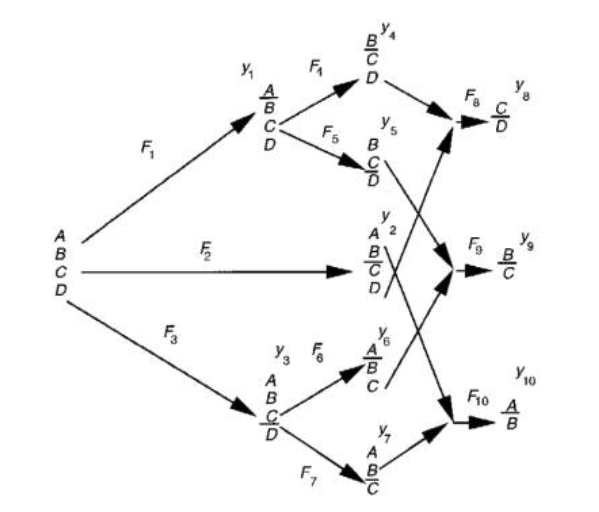
\includegraphics[width=0.50\textwidth]{images/prob2_superstructure.png}}
  \caption{Problem 2 superstructure}
  \label{fig:prob2_superstructure}
\end{figure}

In which the total cost of a distillation column was calculated as follows:

\[
\text{cost}_k = \alpha_k + \beta_k F_k + \gamma_{\text{Hot}} Q_k^{\text{Hot}} + \gamma_{\text{Cold}} Q_k^{\text{Cold}},
\]

where:
\begin{itemize}
    \item $\alpha_k$ represents a fixed capital cost,
    \item $\beta_k$ represents the variable investment cost,
    \item $\gamma_{\text{Hot}}$/$\gamma_{\text{Cold}}$ is the cost of hot/cold utilities,
    \item $Q_k^{\text{Hot}}$/$Q_k^{\text{Cold}}$ is the total demand of hot and cold utilities (assume they are equal).
\end{itemize}

Considering an initial feed of $1000$ Kmol/h, and a composition of the feed stream (mole fraction) of $A=0.15$, $B=0.3$, $C=0.35$, and $D=0.2$, and the following data in Figure~\ref{fig:prob2_table}:

\begin{figure}[htbp]
  \centerline{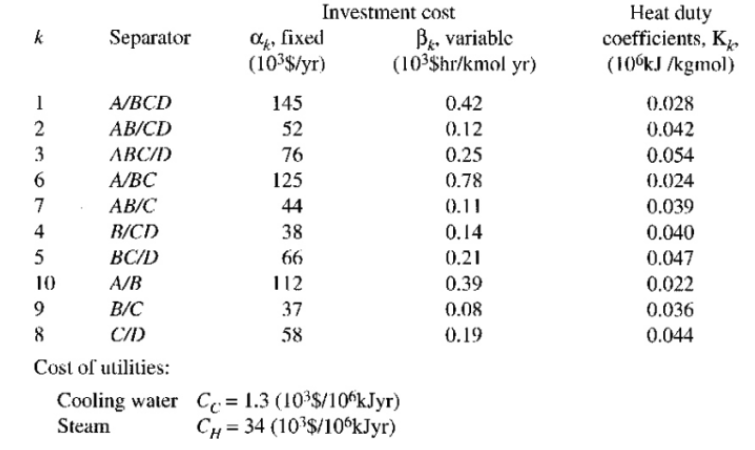
\includegraphics[width=0.75\textwidth]{images/prob2_table.png}}
  \caption{Problem 2 Data table}
  \label{fig:prob2_table}
\end{figure}

\[
\begin{array}{|c|c|c|c|c|}
\hline
\text{Scenario} & \text{Probability} & \gamma_{\text{Hot}} \, (10^3 \, \$/10^6 \, \text{KJ-y}) & \gamma_{\text{Cold}} \, (10^3 \, \$/10^6 \, \text{KJ-y}) \\
\hline
1 & 0.025 & 0.1 & 3 \\
2 & 0.05 & 0.1 & 10 \\
3 & 0.1 & 0.1 & 34 \\
4 & 0.15 & 1.3 & 3 \\
5 & 0.35 & 1.3 & 10 \\
6 & 0.15 & 1.3 & 34 \\
7 & 0.1 & 3 & 3 \\
8 & 0.05 & 3 & 10 \\
9 & 0.025 & 3 & 34 \\
\hline
\end{array}
\]

Unlike the previous case, assume that the parameters $\gamma_{\text{Hot}}$ and $\gamma_{\text{Cold}}$ are known with uncertainty. The probability of occurrence in different scenarios is as follows:




Formulate a stochastic optimization problem in GAMS and solve the problem.

\textbf{Solution:}
\[
\text{minimize} \quad \sum_{s \in S} p_s \cdot \left( \sum_{k=1}^{10} \left( \alpha_k y_k + \beta_k x_k + \gamma_{\text{Hot},s} Q_k^{\text{Hot}} + \gamma_{\text{Cold},s} Q_k^{\text{Cold}} \right) \right)
\]
\[
\text{subject to:}
\]
\[
\begin{aligned}
    & \text{Flow balance constraints (as defined in the problem)} \\
    & \text{Binary constraints for y variables} \\
    & \text{Big-M constraints for x variables} \\
    & \text{Supply and demand constraints} \\
    & \text{Non-negativity constraints for x variables.}
\end{aligned}
\]

We can rearrange the summations 
\[
\text{minimize} \quad \sum_{k=1}^{10} \left( \alpha_k y_k + \beta_k x_k \right) + \sum_{s \in S} p_s \cdot \sum_{k=1}^{10} \left( \gamma_{\text{Hot},s} Q_k^{\text{Hot}} + \gamma_{\text{Cold},s} Q_k^{\text{Cold}} \right)
\]

Previously, in HW5 I didn't successfully incorporate the $Q$ and $\gamma$ values.
Here, the $\gamma$ values are provided per scenario.
I believe the $Q$ values are equal to the amount of flow passing through the distillation column times the heat duty coefficients.
So, using the same variables $y$ and $x$ per distillation column that I had previously, we have the below full problem:


\[
    \text{minimize} \quad \sum_{k=1}^{10} \left( \alpha_k y_k + \beta_k x_k \right) + \sum_{s \in S} p_s \cdot \sum_{k=1}^{10} \left( \gamma_{\text{Hot},s} K_k x_k + \gamma_{\text{Cold},s} K_k x_k \right)
\]
\[
\text{subject to:}
\]
\[
\begin{aligned}
    & \text{Flow balance constraints (as defined in the problem)} \\
    & \text{Binary constraints for y variables} \\
    & \text{Big-M constraints for x variables} \\
    & \text{Supply and demand constraints} \\
    & \text{Non-negativity constraints for x variables.}
\end{aligned}
\]

There are no constraints affected by the uncertainty in the $\gamma$ values.
Therefore, we solve the same problem as previously but augment the objective function to include this uncertainty.
For simplicity, we also split the first section $\sum_{k=1}^{10} \left( \alpha_k y_k + \beta_k x_k \right)$ into $z_1$ as the first stage component and the rest $\sum_{s \in S} p_s \cdot \sum_{k=1}^{10} \left( \gamma_{\text{Hot},s} K_k x_k + \gamma_{\text{Cold},s} K_k x_k \right)$ as the second stage component $z_2$.
Now, $z_T = z_1 + z_2$ is the total objective component.

Another rearrangement we do for simplicity is factoring out the $K x $ term in the second stage component.

\[
    \text{minimize} \quad \sum_{k=1}^{10} \left( \alpha_k y_k + \beta_k x_k \right) + \sum_{k=1}^{10} K_k x_k \sum_{s \in S} p_s \cdot  \left( \gamma_{\text{Hot},s}  + \gamma_{\text{Cold},s} \right)
\]

Since this parameter $\sum_{s \in S} p_s \cdot  \left( \gamma_{\text{Hot},s}  + \gamma_{\text{Cold},s} \right)$ is only comprised of parameters, we can actually calculate a new parameter as the expectation of this term.
Instead of incorporating this into the GAMs, I created a new parameter $E[\gamma] = \sum_{s \in S} p_s \cdot  \left( \gamma_{\text{Hot},s}  + \gamma_{\text{Cold},s} \right)$ and use that to solve the stochastic program below
\[
    \text{minimize} \quad \sum_{k=1}^{10} \left( \alpha_k y_k + \beta_k x_k \right) + \sum_{k=1}^{10} K_k x_k E[\gamma]
\]
\[
\text{subject to:}
\]
\[
\begin{aligned}
    & \text{Flow balance constraints (as defined in the problem)} \\
    & \text{Binary constraints for y variables} \\
    & \text{Big-M constraints for x variables} \\
    & \text{Supply and demand constraints} \\
    & \text{Non-negativity constraints for x variables.}
\end{aligned}
\]

This Python script was used to find the expected gamma:
\begin{verbatim}
# Define the data
scenarios = [
    {"probability": 0.025, "gamma_hot": 0.1, "gamma_cold": 3},
    {"probability": 0.05, "gamma_hot": 0.1, "gamma_cold": 10},
    {"probability": 0.1, "gamma_hot": 0.1, "gamma_cold": 34},
    {"probability": 0.15, "gamma_hot": 1.3, "gamma_cold": 3},
    {"probability": 0.35, "gamma_hot": 1.3, "gamma_cold": 10},
    {"probability": 0.15, "gamma_hot": 1.3, "gamma_cold": 34},
    {"probability": 0.1, "gamma_hot": 3, "gamma_cold": 3},
    {"probability": 0.05, "gamma_hot": 3, "gamma_cold": 10},
    {"probability": 0.025, "gamma_hot": 3, "gamma_cold": 34},
]

# Calculate the summation
summation = sum(
    scenario["probability"] * (scenario["gamma_hot"] + scenario["gamma_cold"])
    for scenario in scenarios
)

# Print the result
print(f"The summation of the gammas times the probability is: {summation:.3f}")
>>> The summation of the gammas times the probability is: 16.062
\end{verbatim}

\subsection{Optimal Solution}
This section will highlight the optimal solution that was found in GAMS.
Section~\ref{prob2_code} has the code that was ran in GAMS
The GAMS output results in this optimal solution:

\begin{table}[htbp]
\centering
\caption{Optimization Results}
\label{tab:optimization_results}
\begin{tabular}{|l|r|r|r|r|}
\hline
\textbf{Variable} & \textbf{Lower} & \textbf{Level} & \textbf{Upper} & \textbf{Marginal} \\ \hline
z\_first\_stage   & -INF           & 622.0000       & +INF           & .                 \\ \hline
z\_second\_stage  & -INF           & 11869.8180     & +INF           & .                 \\ \hline
z\_total          & -INF           & 12491.8180     & +INF           & .                 \\ \hline
x\_1              & .              & .              & +INF           & .                 \\ \hline
x\_2              & .              & 1000.0000      & +INF           & .                 \\ \hline
x\_3              & .              & .              & +INF           & .                 \\ \hline
x\_4              & .              & .              & +INF           & 7.2048            \\ \hline
x\_5              & .              & .              & +INF           & 7.6591            \\ \hline
x\_6              & .              & 450.0000       & +INF           & .                 \\ \hline
x\_7              & .              & 550.0000       & +INF           & .                 \\ \hline
x\_8              & .              & .              & +INF           & 3.9949            \\ \hline
x\_9              & .              & .              & +INF           & 6.4742            \\ \hline
x\_10             & .              & .              & +INF           & 7.4573            \\ \hline
x\_11             & .              & .              & +INF           & 5.8623            \\ \hline
x\_12             & .              & .              & +INF           & 5.8623            \\ \hline
x\_13             & .              & .              & +INF           & 3.7236            \\ \hline
y\_1              & .              & .              & 1.0000         & -7207.4580        \\ \hline
y\_2              & .              & 1.0000         & 1.0000         & 52.0000           \\ \hline
y\_3              & .              & .              & 1.0000         & -3270.3380        \\ \hline
y\_4              & .              & .              & 1.0000         & 125.0000          \\ \hline
y\_5              & .              & .              & 1.0000         & 44.0000           \\ \hline
y\_6              & .              & .              & 1.0000         & 38.0000           \\ \hline
y\_7              & .              & .              & 1.0000         & 66.0000           \\ \hline
y\_8              & .              & 1.0000         & 1.0000         & 112.0000          \\ \hline
y\_9              & .              & .              & 1.0000         & 37.0000           \\ \hline
y\_10             & .              & 1.0000         & 1.0000         & 58.0000           \\ \hline
\end{tabular}
\end{table}

The written explanation of this solution is that 1000 moles are sent to distillation column 2.
It is then split into A and B on top and C and D on bottom where C and D are split by column 10 and A and B are split by column 8.

\subsection{Problem 2 GAMS Code}
\label{prob2_code}
Below is the code that was ran in GAMS
\begin{verbatim}
* I know this is terribly verbose and I should be using sets
* but I haven't been able to get that logic to work

Scalars
f_a /0.15/
f_b /0.30/
f_c /0.35/
f_d /0.20/
S /1000/
    a_1 / 145 /, b_1 / 0.42 /,
    a_2 / 52  /, b_2 / 0.12 /,
    a_3 / 76  /, b_3 / 0.25 /,
    a_4 / 125 /, b_4 / 0.78 /,
    a_5 / 44  /, b_5 / 0.11 /,
    a_6 / 38  /, b_6 / 0.14 /,
    a_7 / 66  /, b_7 / 0.21 /,
    a_8 / 112 /, b_8 / 0.39 /,
    a_9 / 37  /, b_9 / 0.08 /,
    a_10 / 58 /, b_10 / 0.19 /,
K_1 / 0.028 /
K_2 / 0.042 /
K_3 / 0.054 /
K_6 / 0.024 /
K_7 / 0.039 /
K_4 / 0.040 /
K_5 / 0.047 /
K_10 / 0.022 /
K_9 / 0.036 /
K_8 / 0.044 /
E_gamma / 16.062 /
;
Variables
z_first_stage
z_second_stage
z_total
;
Positive Variables
x_1
x_2
x_3
x_4
x_5
x_6
x_7
x_8
x_9
x_10
x_11
x_12
x_13
;
Binary Variables
y_1
y_2
y_3
y_4
y_5
y_6
y_7
y_8
y_9
y_10
;
Equations
    bin_constraint_1
    bin_constraint_2
    bin_constraint_3
    bin_constraint_4
    bin_constraint_5
    bin_constraint_6
    bin_constraint_7
    bin_constraint_8
    bin_constraint_9
    bin_constraint_10
    bin_constraint_11
    bigm_constraint_1_1
    bigm_constraint_1_4
    bigm_constraint_1_5
    bigm_constraint_2_2
    bigm_constraint_2_6
    bigm_constraint_2_7
    bigm_constraint_3_3
    bigm_constraint_3_8
    bigm_constraint_3_9
    bigm_constraint_4_4
    bigm_constraint_4_10
    bigm_constraint_5_5
    bigm_constraint_5_11
    bigm_constraint_6_8
    bigm_constraint_6_12
    bigm_constraint_7_9
    bigm_constraint_7_13
    bigm_constraint_8_6
    bigm_constraint_8_10
    bigm_constraint_9_11
    bigm_constraint_9_12
    bigm_constraint_10_7
    bigm_constraint_10_13
    flow_constraint_7
    flow_constraint_6
    flow_constraint_5
    flow_constraint_4
    flow_constraint_3
    flow_constraint_2_lower
    flow_constraint_2_upper
    flow_constraint_1
    supply_constraint
    integer_cut
    first_stage_objective
    second_stage_objective
    total_objective
;
bin_constraint_1..      y_1 + y_2 + y_3 =e= 1;
bin_constraint_2..      1 - y_1 + y_4 + y_5 =g= 1;
bin_constraint_3..      1 - y_1 + 1 - y_4 + 1 - y_5 =g= 1;
bin_constraint_4..      1 - y_2 + y_8 =g= 1;
bin_constraint_5..      1 - y_2 + y_10 =g= 1;
bin_constraint_6..      1 - y_3 + y_6 + y_7 =g= 1;
bin_constraint_7..      1 - y_3 + 1 - y_6 + 1 - y_7 =g= 1;
bin_constraint_8..      1 - y_4 + y_8 =g= 1;
bin_constraint_9..      1 - y_5 + y_9 =g= 1;
bin_constraint_10..     1 - y_6 + y_9 =g= 1;
bin_constraint_11..     1 - y_7 + y_10 =g= 1;

bigm_constraint_1_1..  x_1  =l= S * y_1;
bigm_constraint_1_4..  x_4  =l= S * y_1;
bigm_constraint_1_5..  x_5  =l= S * y_1;

bigm_constraint_2_2..  x_2  =l= S * y_2;
bigm_constraint_2_6..  x_6  =l= S * y_2;
bigm_constraint_2_7..  x_7  =l= S * y_2;

bigm_constraint_3_3..  x_3  =l= S * y_3;
bigm_constraint_3_8..  x_8  =l= S * y_3;
bigm_constraint_3_9..  x_9  =l= S * y_3;

bigm_constraint_4_4..  x_4  =l= S * y_4;
bigm_constraint_4_10.. x_10 =l= S * y_4;

bigm_constraint_5_5..  x_5  =l= S * y_5;
bigm_constraint_5_11.. x_11 =l= S * y_5;

bigm_constraint_6_8..  x_8  =l= S * y_6;
bigm_constraint_6_12.. x_12 =l= S * y_6;

bigm_constraint_7_9..  x_9  =l= S * y_7;
bigm_constraint_7_13.. x_13 =l= S * y_7;

bigm_constraint_8_6..  x_6  =l= S * y_8;
bigm_constraint_8_10.. x_10 =l= S * y_8;

bigm_constraint_9_11.. x_11 =l= S * y_9;
bigm_constraint_9_12.. x_12 =l= S * y_9;

bigm_constraint_10_7.. x_7  =l= S * y_10;
bigm_constraint_10_13.. x_13 =l= S * y_10;

flow_constraint_7..        x_13 =e= (1 - f_c) / (1 - f_d) * x_9;
flow_constraint_6..        x_12 =e= (1 - f_a) / (1 - f_d) * x_8;
flow_constraint_5..        x_11 =e= (1 - f_d) / (1 - f_a) * x_5;
flow_constraint_4..        x_10 =e= (1 - f_b) / (1 - f_a) * x_4;
flow_constraint_3..        x_9 + x_8 =e= (1 - f_d) * x_3;
flow_constraint_2_lower..  x_7 =e= (1 - f_a - f_b) * x_2;
flow_constraint_2_upper..  x_6 =e= (1 - f_c - f_d) * x_2;
flow_constraint_1..        x_5 + x_4 =e= (1 - f_a) * x_1;

supply_constraint.. x_1 + x_2 + x_3 =e= S;

integer_cut.. y_3 =e= 0;

first_stage_objective..
z_first_stage =e=
    a_1*y_1 + b_1*x_1 +
    a_2*y_2 + b_2*x_2 +
    a_3*y_3 + b_3*x_3 +
    a_4*y_4 + b_4*x_4 +
    a_5*y_5 + b_5*x_5 +
    a_6*y_6 + b_6*x_8 +
    a_7*y_7 + b_7*x_9 +
    a_8*y_8 + b_8*(x_6+x_10) +
    a_9*y_9 + b_9*(x_11+x_12) +
    a_10*y_10 + b_10*(x_7+x_13);
    
second_stage_objective..
z_second_stage =e= E_gamma * 10 * (
    K_1 * x_1 +
    K_2 * x_2 +
    K_3 * x_3 +
    K_4 * x_4 +
    K_5 * x_5 +
    K_6 * x_8 +
    K_7 * x_9 +
    K_8 * (x_6 + x_10) +
    K_9 * (x_11 + x_12) +
    K_10 * (x_7 + x_13)
);

total_objective..
z_total =e= z_first_stage + z_second_stage;

Model Superstructure / all /;
solve Superstructure using MIP minimizing z_total;
\end{verbatim}
\end{document}